\appendix
\appendixpage
\addappheadtotoc





\chapter{Extension of scalars}





\section{Definition and universal property}


Let $L/k$ be a field extension. For a $k$-vector space $V$ we define
\[
 V_L := L \otimes_k V.
\]
Then $V_L$ is a $L$-vector space via
\[
 \lambda \cdot (l \otimes v) = (\lambda l) \otimes v
\]
for all $\lambda \in L$. To see that this multiplication is well-defined notice that for every $\lambda \in L$ the multiplication with $\lambda$ in $L$, namely
\[
 \pi_\lambda : L \to L, l \mapsto \lambda l,
\]
is $L$-linear and thus $k$-linear. The multiplication with $\lambda \in L$ as defined above is simply given by $\pi_\lambda \otimes \id_V$.

Given $k$-vector spaces $V$ and $W$ and a $k$-linear map $f : V \to W$. We get a $k$-linear map
\[
 f_L := \id_L \otimes f : V_L \to W_L.
\]
It is easy to check that $f_L$ is also $L$-linear. Therefore we can understand the extension of scalars as a functor from $\cVect{k}$ to $\cVect{L}$ which associates any $k$-vector space $V$ with $V_L$ and any $k$-linear map $f : V \to W$ with $f_L : V_L \to W_L$.

For any $k$-vector space $V$ we have a $k$-linear inclusion
\[
 \can_V : V \hookrightarrow V_L, v \mapsto 1 \otimes v.
\]


\begin{thrm}[Universal property of the extension of scalars]
 Let $V$ be a $k$-vector space. Then for every $L$-vector space $W$ we have a natural isomorphism of $k$-vector spaces
 \[
  \beta_W: \Hom_L(V_L, W) \to \Hom_k(V,W), f \mapsto f \circ \can_V.
 \]
 This property defines $V_L$ uniquely up to unique isomorphsm: If $V'$ is an $L$-vector space and $\iota : V \to V'$ a $k$-linear map such that
 \[
  \alpha_W : \Hom_L(V', W) \to \Hom_k(V,W), f \mapsto f \circ \iota
 \]
 is an isomorphism of $k$-vector spaces for every $L$-vector space $W$ then there exists a unique isomorphism of $L$-vector spaces
 \[
  \phi : V_L \to V'
 \]
 such that the diagram
 \begin{center}
  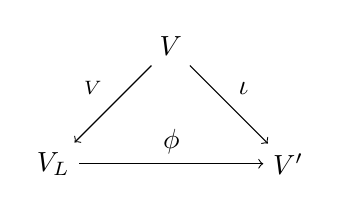
\begin{tikzpicture}[node distance = 6em, auto]
   \node (V) {$V$};
   \node (V_L) [below left of = V] {$V_L$};
   \node (V')  [below right of = V] {$V'$};
   \draw[->] (V) to node[swap] {$\can_V$} (V_L);
   \draw[->] (V) to node {$\iota$} (V');
   \draw[->] (V_L) to node {$\phi$} (V');
  \end{tikzpicture}
 \end{center}
 commutes.
\end{thrm}


That the $\beta_W$ are ``natural'' isomorphisms means the following: Fixing a $k$-vector space $V$ we have two functors
\[
 F_1, F_2 : \cVect{L} \to \cVect{k}
\]
where $F_1(W) := \Hom_L(V_L,W)$ for every $L$-vector space $W$ and for every $L$-linear map $f : W \to W'$
\[
 F_1(f) : \Hom_L(V_L, W) \to \Hom_L(V_L, W'), h \mapsto f \circ h,
\]
as well as $F_2(W) := \Hom_k(V,W)$ for every $L$-vector space $W$ and for every $L$-linear map $f : W \to W'$
\[
 F_2(f) : \Hom_k(V,W) \to \Hom_k(V,W'), h \mapsto f \circ h.
\]
The claim is that the $\beta_W$ form an natural isomorphism from $F_1$ to $F_2$, i.e. they form a natural transformation from $F_1$ to $F_2$ and $\beta_W$ is an isomorphism for every $L$-vector space $W$.


\begin{proof}
 We will start by proving that $\beta_W$ is an isomorphism of $k$-vector spaces for every $L$-vector space $W$. For this we fix an $L$-vector space $W$. It is clear that $\Phi := \beta_W$ is well-defined and $k$-linear. To show that $\Phi$ is an isomorphism we will construct an inverse as
 \[
  \Psi : \Hom_k(V,W) \to \Hom_L(V_L, W), g \mapsto \left( (\lambda \otimes v) \mapsto \lambda g(v) \right).
 \]
 That $\Psi(g)$ is well-defined and $k$-linear for every $g \in \Hom_k(V,W)$ follows from the fact that the map
 \[
  L \times V \to W, (\lambda, v) \mapsto \lambda g(v)
 \]
 is well-defined and $k$-bilinear. That $\Psi(g)$ is also $L$-linear is clear. That $\Psi$ itself is also $k$-linear is also clear.
 
 Since for all $f \in \Hom_L(V_L,W), \lambda \in L, v \in V$
 \begin{align*}
   &\,(\Psi \Phi)(f)(\lambda \otimes v) \\
  =&\,\Psi(\Phi(f))(\lambda \otimes v)
  =   \Psi(f \circ \can_V)(\lambda \otimes v) \\
  =&\,\lambda (f \circ \can_V)(v)
  =   \lambda f(\can_V(v)) \\
  =&\,\lambda f(1 \otimes v)
  =   f (\lambda \otimes v)
 \end{align*}
 we have $\Psi \Phi = \id_{\Hom_L(V_L, W)}$ and since for all $g \in \Hom_k(V,W), v \in V$
 \begin{align*}
  (\Phi \Psi)(g)(v)
  &= \Phi(\Psi(g))(v)
  = (\Psi(g) \circ \can_V)(v) \\
  &= \Psi(g)(\can_V(v))
  = \Psi(g)(1 \otimes v) \\
  &= g(v)
 \end{align*}
 we have $\Phi \Psi = \id_{\Hom_k(V,W)}$.
 
 Next we will show that the $\beta_W$ are natural isomorphisms. For this we need to check that for all $L$-vector spaces $W$ and $W'$ and every $L$-linear map \mbox{$f : W \to W'$} the diagram
 \begin{center}
  \tikzsetnextfilename{naturalisomorphism}
  \begin{tikzpicture}[node distance = 6em, auto]
   \node (HomLW) {$\Hom_L(V_L, W)$};
   \node (HomLW') [right = 6em of HomLW] {$\Hom_L(V_L, W')$};
   \node (HomkW) [below of = HomLW] {$\Hom_k(V,W)$};
   \node (HomkW') [below of = HomLW'] {$\Hom_k(V,W')$};
   \draw[->] (HomLW) to node {$F_1(f)$} (HomLW');
   \draw[->] (HomkW) to node[swap] {$F_2(f)$} (HomkW');
   \draw[->] (HomLW) to node[swap] {$\beta_W$} (HomkW);
   \draw[->] (HomLW') to node {$\beta_{W'}$} (HomkW');
  \end{tikzpicture}
 \end{center}
 commutes, where $F_1$ and $F_2$ are defined as in the previous explanation. This is clear, since $F_1(f)$ and $F_2(f)$ are precomposing with $f$ and $\beta_W$ and $\beta_{W'}$ are composing with $\can_V$, and therefore for all $h \in \Hom_L(V_L, W)$
 \begin{align*}
   &\, (F_2(f) \circ \beta_W)(h)
  =    F_2(f)(\beta_W(h)) \\
  =&\, F_2(f)(h \circ \can_V)
  =    f \circ (h \circ \can_V) \\
  =&\, (f \circ h) \circ \can_V
  =    \beta_{W'}(f \circ h) \\
  =&\, \beta_{W'}(F_1(f)(h))
  =    (\beta_{W'} \circ F_1(f))(h).
 \end{align*}
 
 All that’s left to show is that property defines $V_L$ uniquely up to unique isomorphism. To prove this let $V'$ be an $L$-vector space together with a $k$-linear map $\iota : V \to V'$ such that for every $L$-vector space $W$ the map
 \[
  \alpha_W : \Hom_L(V', W) \to \Hom_k(V, W), f \mapsto f \circ \iota
 \]
 is an isomorphism of $k$-vector spaces.
 
 First we notice that
 \[
  \Hom_L(V_L, V_L) \cong \Hom_k(V, V_L), f \mapsto f \circ \can_V.
 \]
 Therefore there exists exactly one $f \in \Hom_L(V_L, V_L)$ with $f \circ \can_V = \can_V$. It is clear that $f = \id_{V_L}$. In the same way we find that $g \in \Hom_L(V', V')$ with $g \circ \iota = \iota$ if and only if $g = \id_{V'}$.
 
 Next we notice that
 \[
  \Hom_L(V_L, V') \cong \Hom_k(V, V'), f \mapsto f \circ \can_V.
 \]
 Therefore there exists a unique $L$-linear map $\phi \in \Hom_L(V_L, V')$ such that \mbox{$\iota = \phi \circ \can_V$}. All that’s left to check is that $\phi$ is an isomorphism. For this we find in same way that there exists a unique $L$-linear map $\psi \in \Hom_L(V', V_L)$ with $\can_V = \psi \circ \iota$. Since
 \[
  \phi \psi \circ \iota = \phi \circ \can_V = \iota
 \]
 as well as
 \[
  \psi \phi \circ \can_V= \psi \circ \iota = \can_V
 \]
 we find by the previous observations that $\phi \psi = \id_{V'}$ and $\psi \phi = \id_{V_L}$.
\end{proof}


Another important observation is that $\can_V$ maps a $k$-basis of $V$ to a $L$-basis of $V_L$. In particular $\dim_k V = \dim_L V_L$.


\begin{lem}
 Let $V$ be a $k$-vector space and $(v_i)_{i \in I}$ a $k$-basis of $V$. Then $(1 \otimes v_i)_{i \in I}$ is an $L$-basis of $V_L$.
\end{lem}
\begin{proof}
 First we show that $(1 \otimes v_i)_{i \in I}$ is linearly independent. For this let $F$ be the free vector space of $I$ over $L$ and $e_i \in F$ the element corresponding to $i \in I$. Because $(v_i)_{i \in I}$ is a $k$-basis of $V$ there exists an unique $k$-linear map $f : V \to F$ with $f(v_i) = e_i$ for all $i \in I$. By the universal property of extension of scalars there exists a unique $L$-linear map $g : V_L \to F$ with $g \circ \can_V = f$ and therefore
 \[
  g(1 \otimes v_i) = (g \circ \can_V)(v_i) = f(v_i) = e_i
 \]
 for all $i \in I$. Since $(e_i)_{i \in I}$ is linearly independent it follows that $(1 \otimes v_i)_{i \in I}$ is linearly independent.
 
 To show that $\{1 \otimes v_i\}_{i \in I}$ generates $V_L$ we notice that
 \[
  \vspan_k \{1 \otimes v_i\}_{i \in I}
  = \im \can_V
  = \{1 \otimes v \mid v \in V\}.
 \]
 Since the simple tensors (i.e. the tensors $\lambda \otimes v$ with $\lambda \in L$ and $v \in V$) generate $V_L$ and $\lambda \otimes v = \lambda(1 \otimes v)$ for all $\lambda \in L, v \in V$ we find that
 \begin{align*}
  V_L
  &= \vspan_L \{\lambda \otimes v \mid \lambda \in L, v \in V\}
  = \vspan_L \{1 \otimes v \mid v \in V\} \\
  &= \vspan_L \vspan_k \{1 \otimes v_i \mid i \in I\}
  = \vspan_L \{1 \otimes v_i \mid i \in I\}.
 \end{align*}
 Therefore $\{1 \otimes v_i\}_{i \in I}$ generate $V_L$.
\end{proof}
















